% !TeX spellcheck = en_US
% !TeX encoding = UTF-8
% !TeX root = ../report.tex

\large

\chapter{Disposition}
\label{chp:disposition}

In these few subsections I will lay out what the context, the goal and the methods of this term paper.

\section{Summary}
Reranking and the use of genetic algorithms are two popular approaches when it comes to implementing  multi-objective recommender systems. In recent articles genetic approaches seem to perform well but show some limitations in regard to the size of the training data sets and the duration of the training itself. The goal of this term paper is to find these limits. A comparison between the two approaches and baseline algorithms (for example matrix factorization or collaborative filtering) will help determine the usefulness of the approaches in question.

\section{Introduction}
Recommender Systems have become a useful tool in the world wide web, both for consumers (users) and producers (service providers). With the help of these Systems, users can find relevant information without having to go through tens of thousands of data points and service providers are able to improve the user experience and even increase revenue. Amazon for example uses recommender systems to recommend products to customers that might interest them, based on user information and what kind of items the user bought in the past.
\newline
A type of recommender systems that have become more relevant lately are multi-objective recommender systems. These systems are trained to include additional optimization goals. Relevance has long been the most relevant metric to quantify the usefulness of recommender systems. But there are other aspects to these system which are not correlated to relevance, for example the diversity and novelty of recommendations to the user. A user might be interested to explore different types of items and not items that are very similar to the ones he already found. 
\newline
There are different approaches to creating systems that produce not only accurate recommendations but also diverse and novel recommendations. One of the older approaches is called reranking. In this approach we first optimize a system on one objective (for example relevance) and rerank the order of produced recommendations based on a second objective (for example diversity). Later approaches introduce genetic algorithms that are able to optimize for multiple objectives at once or neural approaches that use a multi-gradient descent optimization to optimize for multiple goals at once.
\newline
In this term paper we will look at two of these approaches, namely reranking and genetic systems.

\section{Research question}
The research questions to be answered throughout this term paper are the following:: \textbf{\emph{\begin{enumerate}
        \item What are the limits with respect to computational time and processable data set size with the current genetic approaches for multi-objective recommender systems?
        \item Does the performance of these systems justify their limits?
    \end{enumerate}}}
    
\section{Approach}
To find the answers to these questions, recent published reranking and genetic algorithms will be implemented and compared to two baselines, a matrix factorisation and an item-based collaborative filtering approach. A comparison will be made to see which systems perform better and how the training time differs between these approaches.
\newline
The different algorithms will be optimized for two objectives, namely relevance and novelty, two well know optimization goals in the recommender system field. To quantify these goals, we use the recall@R metric shown in equation \ref{eq:recall}, for example found in the work of Liang et al. \cite{liang2018variational} for relevance. The mean self-information@R metric shown in equation \ref{eq:surprisal}, found for example in the work of Zhou et al. \cite{zhou2010solving} will be used to quantify novelty.

\begin{equation} \label{eq:recall}
Recall@R(u,\omega) := \frac{\sum\nolimits_{r=1}^R \mathbb{I}[\omega(r) \in I_u]}{min(M, |I_u|)}
\end{equation}

\begin{equation} \label{eq:surprisal}
Surprisal@R(u,\omega) := \frac{\sum\nolimits_{r=1}^R log_2(\frac{|U|}{k_{\omega(r)}})}{|R|}
\end{equation}

Chai et al. \cite{chai2018immune} and Lin et al. \cite{lin2018multiobjective} both propose genetic algorithms based on collaborative filtering and single value decomposition for multi-objective optimization. One of these approaches will be implemented and tested against a simpler reranking approach proposed by Adomavicius et al. \cite{adomavicius2009toward}.


\section{Data}
To test these assumptions, the MovieLens 1M data set will be used. It is a public data set that contains one million movie ratings from 6000 users on 4000 movies. The use of this public data set ensures the reproducibility of the results of this term paper.
\newline
The users rate the movies on a scale from one to five. These explicit ratings are being converted to binary ratings, \say{zero} meaning the user didn't like the movie or hasn't rated it yet and \say{one} meaning the user enjoyed the movie. This done with a simple transformation so that ratings $>= 3.5$ are converted to $1$ and ratings $<3.5$ are converted to $0$.


\section{Timeline}
The following graphic shows the timeline for the creation of this term paper.


\begin{figure}[htpb]
    \centering
    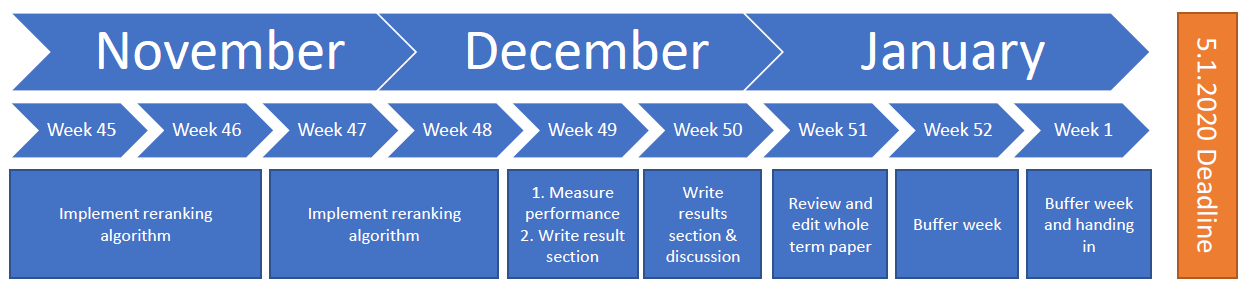
\includegraphics[width=\textwidth]{img/timeline.PNG}
    \caption{Timeline}
    \label{fig:timeline}
\end{figure}

